\documentclass[11pt, a4paper, reqno]{scrartcl}

\usepackage[utf8]{inputenc}
\usepackage{a4wide}
\usepackage{libertine}
\usepackage{graphicx}
\usepackage{listings}
\usepackage{xcolor}
\usepackage{float}
\usepackage{amsmath}
\usepackage{microtype}
\usepackage{hyperref}
\usepackage{pdflscape}

% for latex output of pandas
\usepackage{booktabs}

\begin{document}
    \title{Exercise No. 10}
    \author{David Bubeck, Pascal Becht, Patrick Nisbl\`e}
    \maketitle

    \lstset{
        language=Python,
        backgroundcolor=\color{gray!5},
        numbers=left,
        captionpos=t,
        breaklines=true,
        frame=l,
        xleftmargin=\parindent,
        basicstyle=\footnotesize\sffamily,
        keywordstyle=\bfseries\color{green!40!black},
        commentstyle=\itshape\color{purple!40!black},
        identifierstyle=\color{blue!60!black},
        stringstyle=\color{orange}
    }

    \section*{2 - Probability distribution functions}
   
    	We have given a probability distribution function $p(x)$ in the domain $[0, 		a)$ by
    	\begin{align}
    		p(x) = bx
    	\end{align}
    	Were $b$ is the normalization factor. At first we need to calculate $b$ as 			a fuction of $a$ to normalize the given pdf. Therefore we integrate the pdf 		from $0$ to $a$ which has to be one.
    	\begin{align*}
    		\int_{0}^{a} bx \, dx \overset{!}{=} 1
    	\end{align*}
    	For the solution we obtain
    	\begin{align*}
    		b = \frac{2}{a^2}
    	\end{align*}
    	Our normalized pdf is now
    	\begin{align*}
    		p(x) = \frac{2}{a^2}x
    	\end{align*}
    
     	For the calculation we used a random set of numbers which are uniformly 			distributed between 0 and 1. With the rejection method we calculated 				random numbers which obeyed equation 2.1 for $a = 0.5$. So we generated 			another set of random numbers uniformly distibuted as before to check if
     	\begin{align*}
     		v \leq \frac{p(x)}{g(x)}
     	\end{align*}
     	with
     	\begin{align*}
     		g(x) = \frac{2}{a}
     	\end{align*}
		because $p(x)$ reaches it's maximum at $x = a$
     	
     	
     	\begin{figure}[H]
     		\lstinputlisting[lastline=35]{Exercise10_1.py}
     	\end{figure}

    	Here are the plots for the solutions given with the code above. In figure 1 		is show the histogram with the random number sample and the overplotting 			probability distribution function. In figure 2 is shown the individual 				random numbers which were accepted or rejected by the given algorithm. Also 		for this graph it was chosen a sampling of 10000 which gave us a reasonable 		fit (by eye) as you can see. 
        \begin{figure}
        	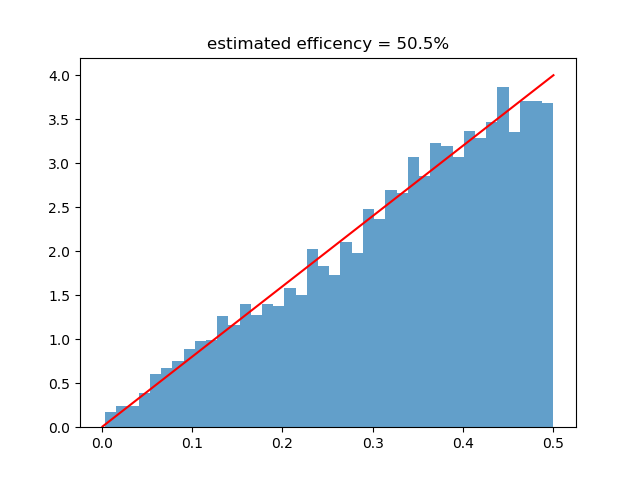
\includegraphics[width=0.67\paperwidth]{pdf.png}
            \caption{histogram for the pdf with overploting equation 2.1}
            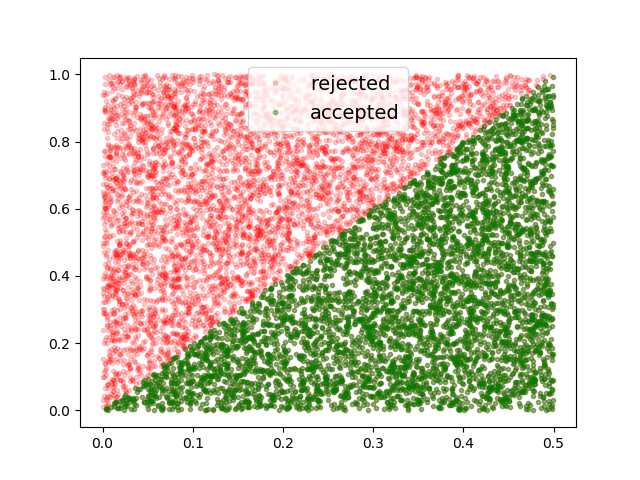
\includegraphics[width=0.67\paperwidth]{accepted_rejected.png}
            \caption{accepted and rejected random numbers}
        \end{figure}
 
 	\newpage
 	
	\section*{3 - Determine $\pi$ with random numbers}
		
		To compute the number $\pi$ we use the function
		\begin{align}
			f(x) = \sqrt{1 - x^2} \;\;\; for \;\;\; 0 \leq x \leq 1
		\end{align}
		Also we using the rejection method as above with a slightly adjustment for 			the further calculation of the accuracy of the result as a function of the 			random number. Furthermore, due to symmetry we only need to sample from the 		upper right corner of the box (one quarter of the circle). In this case the 		fomula to determine $\pi$ can be explicitly written as:
		\begin{align*}
			\frac{pointsInCircle}{totalPoints} = \frac{\pi \cdot L^2}{4 \cdot L^2}
		\end{align*}
        So $\pi$ can be approximated with
        \begin{align*}
        	\pi = \frac{pointsInCircle}{totalPoints} \cdot 4
        \end{align*}
        \newline
        Like above you can see in figure 3 histogram of the random number sample 			which follows the given function. Figure 4 show the accepted and rejected 			values. Also we have an approximation of $\pi$ for this sample of 					$\pi_{approximation} = 3.14404$. This calculation was made with a random 			number sample of 100000.
        \newline
        The graph for the error calculation is shown in figure 5. You can see that 			the accuracy of the result will be better with higher random number sample.
        
        \begin{figure}[H]
     		\lstinputlisting[lastline=56]{Exercise10_2_final.py}
     	\end{figure}
     	
     	\begin{figure}
        	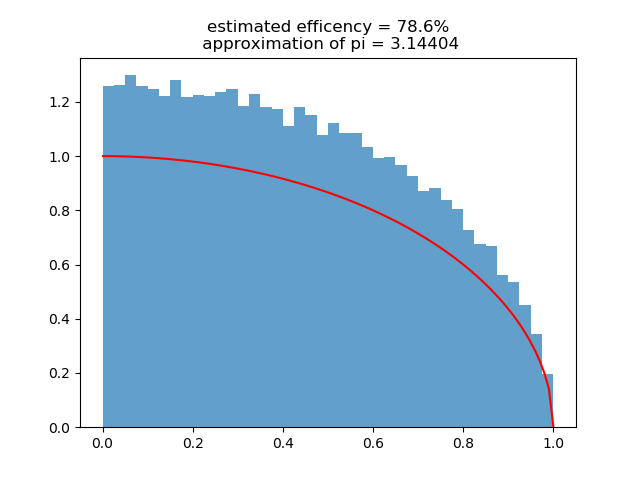
\includegraphics[width=0.43\paperwidth]{pi.png}
            \caption{histogram for the function 2}
            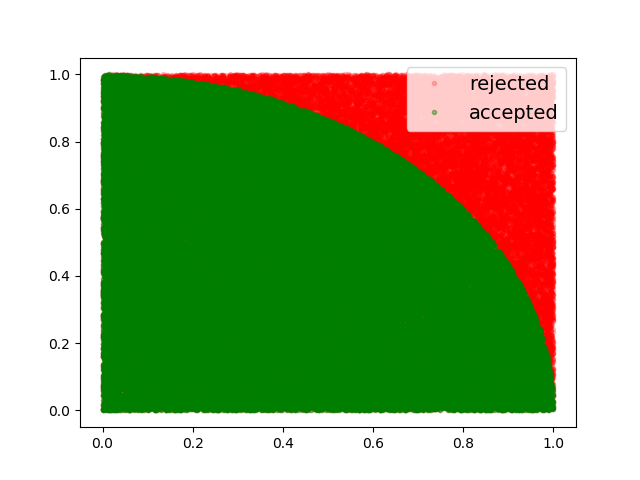
\includegraphics[width=0.43\paperwidth]{accepted_rejected_pi.png}
            \caption{accepted and rejected random numbers}
            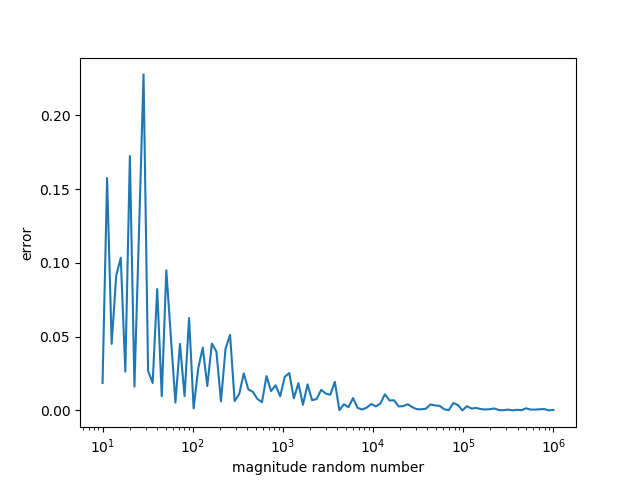
\includegraphics[width=0.43\paperwidth]{error_calculation_pi.png}
            \caption{accuracy of the result as function of the number of samples}
        \end{figure}
        
        
        
		        
\end{document}